\chapter{四个可复现的数值实验}
\label{ch:experiments}
\chaptertakeaway{把理论结论变成可检查的数值判断：解析解是否与建模解一致，哪个约束限制性能，非凸算法是否依赖初值，以及优化误差与估计误差有何区别。}

本章图形由随书 Python 代码实际计算得到。注水和 SINR 可行性模型改编自 CVXPY 的开放案例\cite{cvxpyexamples}；新加入解析解对照、物理单位说明、约束残差、多初值比较和原始数据导出。所有功率均以同一参考功率归一化；$G$ 表示功率增益，$H$ 表示幅度增益，二者不能直接混用。四个实验分别回答不同问题，单次确定性算例用于解释机制，不承担随机信道下的平均性能评估。

\section{注水：不用的信道也是最优解的一部分}

四个正交信道的等效噪声功率取
$\bm\alpha=(1,2,4,8)^\T$，总功率为 $10$。最大化
$R=\sum_{n=1}^{4}\log_2(1+p_n/\alpha_n)$ 后，第四个信道不分配功率。其噪声底高于最优水位，把有限功率先放到前三个信道能获得更高的边际收益。每个信道带宽取 $1\,\mathrm{Hz}$ 时，$R$ 的数值等于总速率（$\mathrm{bit/s}$）；按整个 $4\,\mathrm{Hz}$ 带宽计算的系统频谱效率应为 $R/4$。

由 $\sum_n[\mu-\alpha_n]_+=10$ 得
\begin{equation}
 \mu=\frac{17}{3},\qquad
 \bm p^\star=\left(\frac{14}{3},\frac{11}{3},\frac{5}{3},0\right)^\T.
\end{equation}
代入物理速率公式得到 $R=4.507501\,\mathrm{bit/s}$，等功率分配则为
$4.070037\,\mathrm{bit/s}$。代码通过区间宽度 $10^{-12}$ 的水位二分求解析结构解，并独立调用 CVXPY 求解原凸问题；两者功率分量最大差约 $7.13\times10^{-6}$。通用求解器的目标收敛精度与变量精度并不相同，尤其在最优点附近目标较平坦时，功率误差可以比目标误差大。

\begin{figure}[H]
 \centering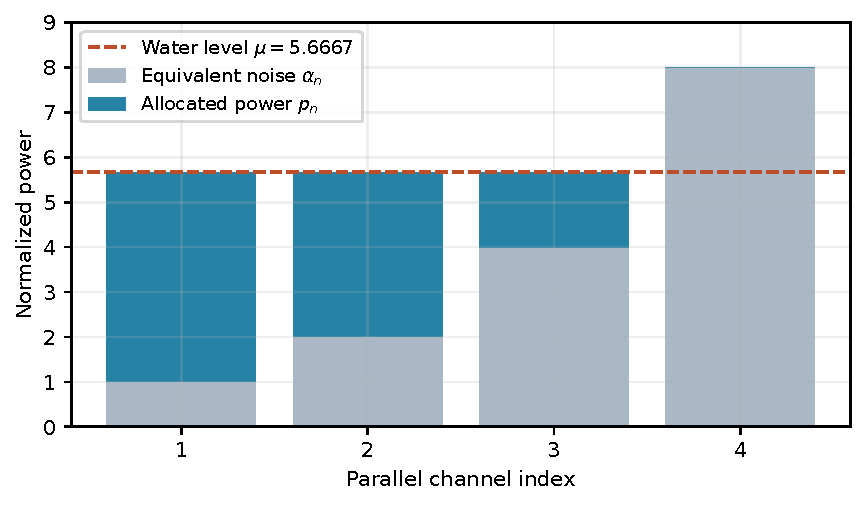
\includegraphics[width=.75\linewidth]{water_filling.pdf}
 \caption{四个单位带宽正交信道的注水分配。灰色为归一化等效噪声功率 $\alpha_n$，蓝色为分配功率 $p_n$，虚线为水位 $\mu=17/3$。总分配功率为 $10$；第四个信道的噪声底超过水位，分配功率为零。}
 \label{fig:water-numeric}
\end{figure}

\section{功率控制：谱半径条件与实际预算共同决定可行性}

三个同频链路的功率增益、噪声功率及预算取
\begin{equation}
 G=\begin{bmatrix}1&.15&.1\\.2&1&.15\\.1&.2&1\end{bmatrix},\qquad
 \sigma_k^2=.1,\quad 0\le p_k\le1,\quad\sum_kp_k\le2.
 \label{eq:numeric-power-data}
\end{equation}
要求所有链路的 SINR 至少为 $2$ 时，最小功率为
\begin{equation}
 \bm p^\star=(.462686567,.537313433,.507462687)^\T.
\end{equation}
此时 $\rho(F)=.602486<1$，三个 SINR 约束均取等号。闭式解
$(I-F)^{-1}\bm\eta$ 与 LP 解的最大分量差为 $2.44\times10^{-12}$；把 LP 解代回原 SINR 不等式、峰值与总功率约束，最大正违约量为 $1.35\times10^{-12}$。

逐步提高共同目标 $\gamma$ 时，总功率预算先限制性能。用闭式最小功率作为可行性判据，从可行下界 $0$ 和不可行上界 $10$ 开始二分，30 次后得到
\begin{equation}
 2.2170723043\le\gamma^\star\le2.2170723137.
\end{equation}
下界对应功率约为 $(.609406,.716203,.674392)^\T$，总和约为 $2$，单用户峰值仍有余量。代码还在此区间两侧各距 $10^{-3}$ 的目标处调用 LP 交叉检查可行与不可行状态；使用该间隔是为避开有限精度求解器对边界附近状态的敏感性。最终窄区间来自闭式判据，并未把求解器状态误当成无限精度证明。

\begin{figure}[H]
 \centering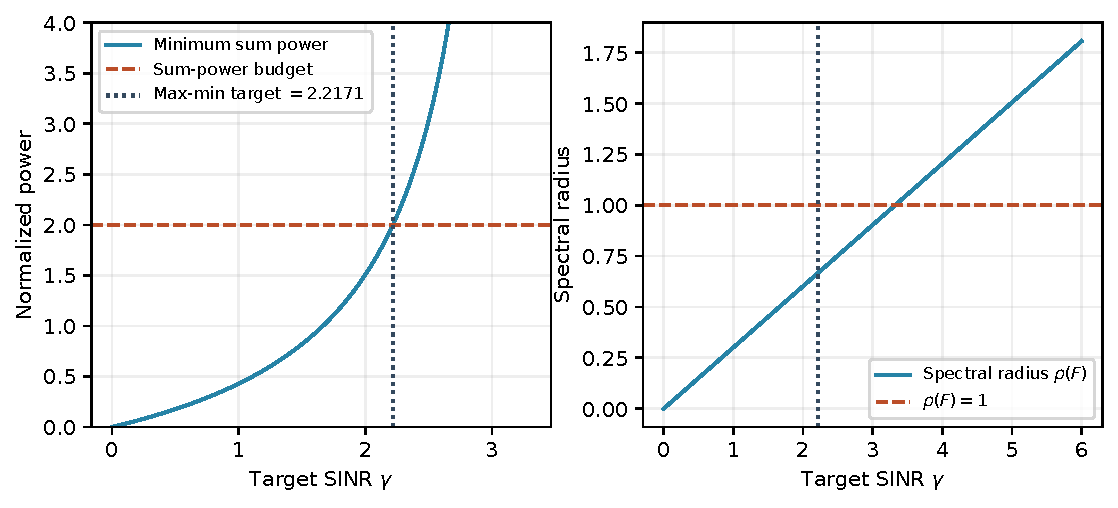
\includegraphics[width=.9\linewidth]{power_control.pdf}
 \caption{式~\eqref{eq:numeric-power-data} 的共同 SINR 目标扫描，步长为 $.02$。左图为仅考虑 SINR 时的最小总功率（纵轴显示到 $4$），水平虚线是总功率预算 $2$；右图为相应 $F$ 的谱半径。竖线标出实际预算下的最大共同 SINR。$\rho(F)<1$ 保证无预算时存在有限功率解；加入功率预算后，可行范围进一步缩小。}
 \label{fig:power-numeric}
\end{figure}

\section{WMMSE：单调上升仍可能到达不同解}

实幅度三用户干扰信道取
\begin{equation}
 H=\begin{bmatrix}1&.8&.3\\.7&1&.6\\.4&.5&1\end{bmatrix},\quad
 \sigma_k^2=.2,\quad \sum_k v_k^2\le3.
\end{equation}
仍采用复基带单位带宽速率模型；实数是本算例对信道系数和幅度的取值限制。这里 $v_k\ge0$ 是发射幅度，功率为 $p_k=v_k^2$；SINR 中的增益为 $|H_{kj}|^2$。三个用户权重均为 $1$，目标为同频链路的和频谱效率
$\sum_k\log_2(1+\SINR_k)$。固定接收器和 MSE 权重后，幅度更新的功率乘子用 80 次二分求得。迭代在相邻目标增量不超过
$10^{-10}\max(1,|R|)$ 时停止，最多 3000 次。

等功率初值和随机种子 $7$ 生成的正初值分别在 59、64 次迭代后到达约
数值 $4.597239615$（单位 bit/s/Hz），对应功率约为
$(1.3618,0,1.6382)^\T$。偏向第二个用户的初始功率
$(.01,2.98,.01)^\T$ 则在 15 次迭代后到达约
$4.000000000\,\mathrm{bit/s/Hz}$。三条轨迹均单调上升，但后者停在性能较低的解；因此“迭代不再改善”不能替代全局最优性证书。

为提供独立参照，代码枚举功率单纯形
$p_1+p_2+p_3=3$ 上步长为 $.02$ 的 11476 个点，最好可行点为
$(1.36,0,1.64)^\T$，目标为 $4.597239011$。只检查总功率取满的点有依据：正噪声下，把任意非零功率向量共同放大至预算边界，会严格改善各活跃链路的 SINR。有限网格给出的是可行目标，即全局最大值的下界；它没有覆盖所有连续功率分配，因而不是最优值上界。

\begin{figure}[H]
 \centering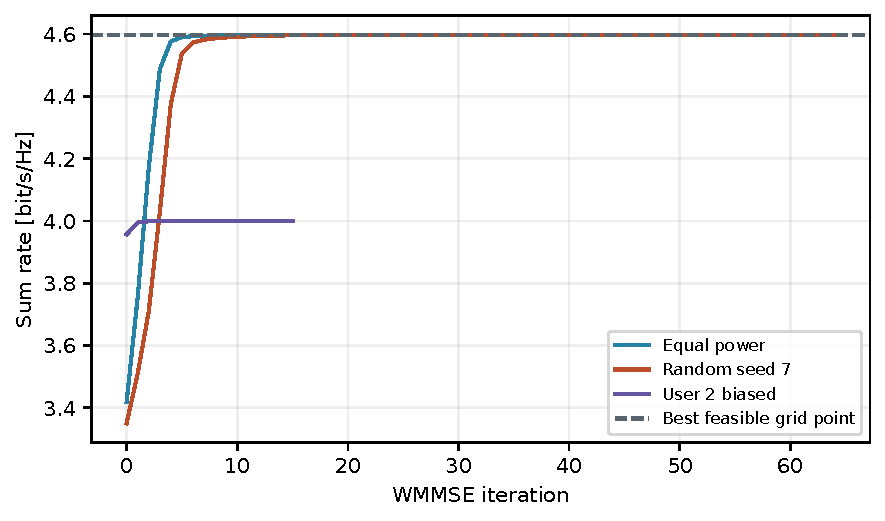
\includegraphics[width=.8\linewidth]{wmmse.pdf}
 \caption{三用户实 SISO 信道的 WMMSE 和频谱效率轨迹。随机初值由种子 $7$ 生成；偏置初值的功率为 $(.01,2.98,.01)^\T$。虚线为步长 $.02$ 的功率网格中最好可行点的目标，仅作数值参照。各条曲线在达到停止条件后结束。}
 \label{fig:wmmse-numeric}
\end{figure}

\section{稀疏估计：目标解得准与信道估得准是两件事}

实信道观测取 $\bm y=A\bm h+\bm n$：$A\in\R^{40\times80}$ 的元素由标准高斯分布生成后逐列归一化，$\bm h$ 只有 5 个非零分量，噪声标准差为 $.02$。所有随机量由同一 NumPy 生成器、种子 $7$ 顺序产生；非零位置及观测矩阵另存于数据文件。求解
\begin{equation}
 \min_{\bm x}\ \frac12\norm{A\bm x-\bm y}_2^2+.06\norm{\bm x}_1.
\end{equation}
ISTA 步长为 $1/L$，其中 $L=\norm{A}_2^2=5.310545$。以近端梯度映射的无穷范数小于 $10^{-8}$ 为停止条件，210 步后目标约为 $.2690157144$，与 CVXPY 参考目标的绝对差约 $1.52\times10^{-11}$；近端梯度映射范数为 $9.31\times10^{-9}$。这一数值证据说明优化问题已被高精度求解。

相对信道估计误差 $\norm{\widehat{\bm h}-\bm h}_2/\norm{\bm h}_2$ 仍约为 $6.71\%$。噪声和 $\ell_1$ 正则化带来的收缩偏差不会随着优化迭代继续增加而消失。选择正则化参数需要考虑噪声与估计任务，单看优化目标下降曲线不足以确定它。

\begin{figure}[H]
 \centering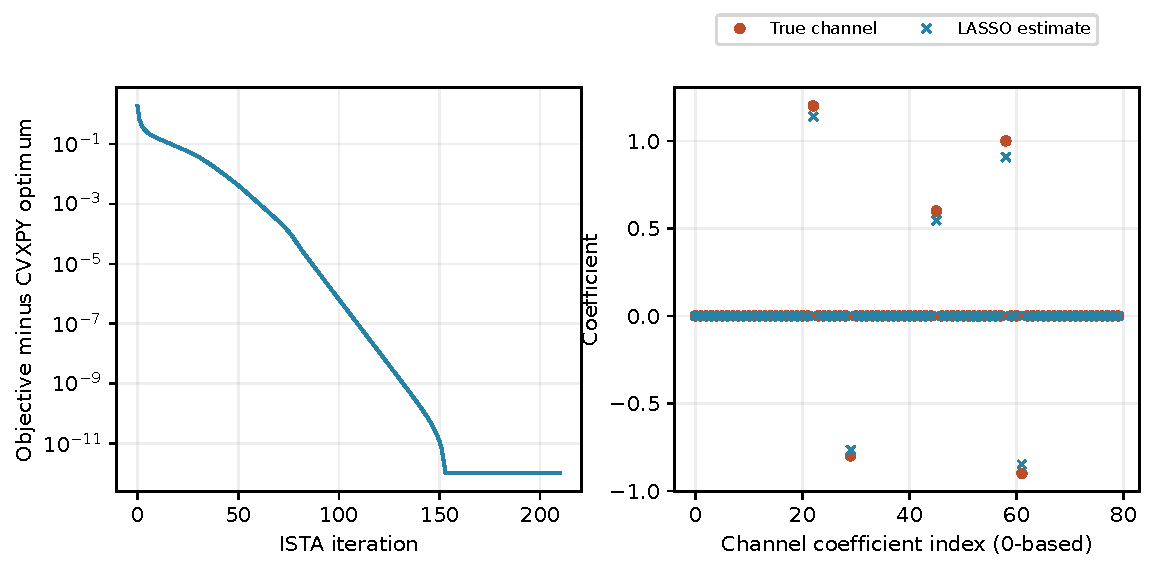
\includegraphics[width=.9\linewidth]{lasso.pdf}
 \caption{种子 $7$ 的稀疏信道估计。左图为 ISTA 目标减去 CVXPY 参考目标，作图时把小于 $10^{-12}$ 的差截至 $10^{-12}$，以容纳数值误差和对数坐标；右图为真实系数与 LASSO 估计，横轴沿用代码的零起始索引。列归一化矩阵尺寸为 $40\times80$，非零系数数目为 5，$\lambda=.06$，噪声标准差为 $.02$。}
 \label{fig:lasso-numeric}
\end{figure}

\section{复现与结果文件}

在已安装依赖的 Python 环境中，从教材根目录执行
\begin{lstlisting}
python code/run_experiments.py
\end{lstlisting}
即可重新生成全部四组图形与数据；编译教材时直接使用已附的 PDF 图，无需运行 Python。代码中包含闭式解对照、功率可行性和 WMMSE/ISTA 单调性断言。若断言不通过，应检查版本与数值状态后再解释图形。

本次运行使用 Python 3.12.14、NumPy 2.3.5、SciPy 1.17.0、CVXPY 1.9.3、Matplotlib 3.10.8 和 CLARABEL 0.11.1。凸子问题的绝对、相对间隙和可行性容差均设为 $10^{-10}$。完整参数与诊断保存在
\texttt{data/results.json}；迭代历史及系数保存在 CSV，稀疏观测输入保存在
\texttt{data/lasso\_input.npz}。版本变化可能影响最后几位数值，判断结论时应同时比较目标、原约束残差和停止准则。
